\chapter{Fundamentação teórica}\label{cap:revisao}

Nesta seção será discutido o funcionamento e as principais características do
LZ77 e do algoritmo aritmético, com o propósito de permitir ao leitor uma
melhor compreensão dos algoritmos utilizados neste trabalho.

\section{Funcionamento do LZ77}\label{sec:LZ77}

O algoritmo de compressão LZ77, proposto por Ziv e Lempel em
1977~\cite{1055714}, pertence à classe dos métodos baseados em dicionário.

O LZ77 consiste em analisar a sequência de entrada de símbolos $S$ pertencentes a um alfabeto finito
$\mathcal{X}$ dividindo-o em partes menores, no qual o comprimento não deve ultrapassar
um valor máximo de $L_{c}$. Além disso, estabelece um esquema de codificação que converte essas subcadeias, 
de forma sequencial, em palavras-código de comprimento fixo $L_{s}$, também sobre o mesmo alfabeto $\mathcal{X}$, garantindo que o processo de decodificação não seja ambíguo~\cite{1055714}.

Para realizar a codificação, temos o algoritmo utiliza uma janela deslizante ou buffer que
percorre a sequência de entrada. Essa janela é dividida em duas regiões
principais:

\begin{itemize}
  \item \textbf{\textit{$S$ ou Search buffer}}: contém a porção já codificada da sequência, correspondendo ao "passado" armazenado, seu tamanho é de $n - L_{s}$
  \item \textbf{\textit{$L$ ou Lookahead buffer}}: contém a porção da sequência que ainda não foi codificada, representando o "futuro" a ser processado, seu tamanho é de $L_{s}$
  \item \textbf{\textit{$W$ ou sliding window}}:  W é o tamanho total da janela. onde:
\[
    W = S + L,
\]
\end{itemize}


Durante a codificação, o algoritmo utiliza um ponteiro de correspondência
(\textit{match pointer}) que percorre o \textit{search buffer} para identificar
o maior prefixo do \textit{lookahead buffer} que também ocorra ali. Quando uma
correspondência é encontrada, ela é codificada como um token $\langle p, \ell,
  x \rangle$, onde:
\begin{itemize}
  \item $p$ (\textit{pointer}): p é o deslocamento dentro da janela (endereçando uma posição anterior no buffer)
  \item $\ell$ (\textit{length}): comprimento da sequência que será codificada limitado a $L_{s}$;
  \item $x$ (\textit{character}): $x \in \mathcal{X}$, é o próximo caractere literal que segue a sequência codificada.
\end{itemize}

A Figura~\ref{fig:Diagrama LZ77} ilustra essa estrutura, destacando as divisões
da janela deslizante e o funcionamento da busca por correspondências.

\begin{figure}[ht]
  \centering
  \caption{Divisão da janela deslizante no algoritmo LZ77}
  \label{fig:Diagrama LZ77}
  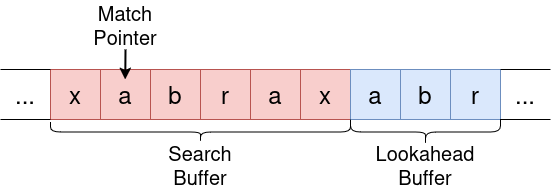
\includegraphics[width=12cm]{figuras/DiagramasTCC-LZ77-template}
  \fonte{Adaptada de \textcite{sayood2012introduction}}
\end{figure}

Este mecanismo permite substituir sequências repetidas por referências a
ocorrências anteriores, resultando em compressões eficazes especialmente para
dados com alta redundância.

% Aqui
\subsection{Exemplo de Codificação com LZ77}\label{sec:LZ77_exemplo}

Nesta seção será demonstrado um exemplo detalhado do funcionamento da janela
deslizante e da representação do token $\langle p, \ell, x \rangle$ utilizados
pelo algoritmo LZ77. 

A sequência a ser codificada é \texttt{"cabracadabrarrarrad"}. Para este exemplo, a janela deslizante possui
um tamanho total fixo de 13 caracteres, com o \textit{lookahead buffer}
definido em 6 caracteres. O estado inicial da janela pode ser visto na
Figura~\ref{fig:Estado_0_LZ77}.

\begin{figure}[htp]
  \centering
  \caption{Estado inicial da janela deslizante no algoritmo LZ77}
  \label{fig:Estado_0_LZ77}
  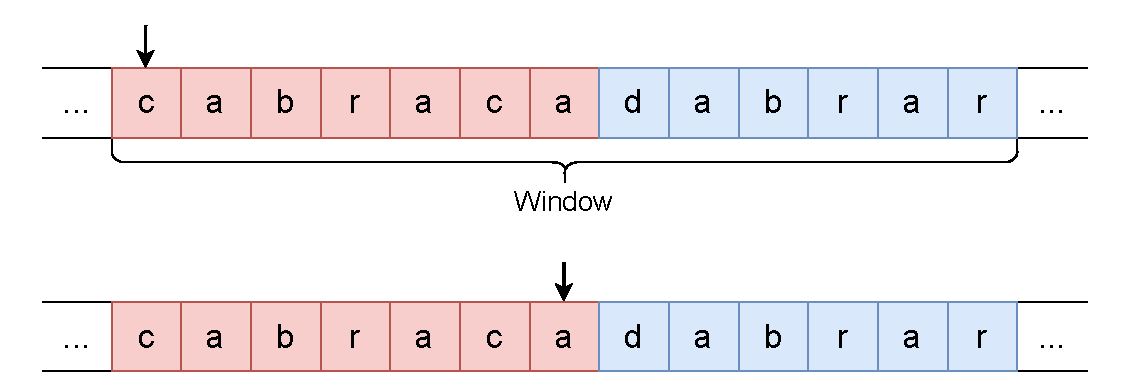
\includegraphics[width=15cm]{figuras/DiagramasTCC-LZ77-Estado-0.pdf}
  \fonte{Adaptada de \textcite{sayood2012introduction}}
\end{figure}

Inicialmente, busca-se no \textit{search buffer} , da esquerda para direita, algum caractere ou sequência
que coincida com o início do \textit{lookahead buffer}. Neste momento,
deseja-se codificar o primeiro caractere do \textit{lookahead buffer}, que é
\texttt{"d"}. Ao observar o \textit{search buffer}, verifica-se que não há
nenhuma correspondência prévia para este caractere. Portanto, o algoritmo gera
o token $\langle 6, 0, \texttt{d} \rangle$, indicando que não houve
correspondência, apesar de o pointer ser 6, o comprimento da sequência
 é 0, assim não fazendo a diferença na codificação, pois não existe cópia sendo feita.

Após esta codificação inicial, a janela deslizante avança uma posição, o que
altera o conteúdo tanto do \textit{search buffer} quanto do \textit{lookahead
  buffer}, conforme mostrado na Figura~\ref{fig:Estado_1_LZ77}.

\begin{figure}[htp]
  \centering
  \caption{Estado da janela após primeira codificação no algoritmo LZ77}
  \label{fig:Estado_1_LZ77}
  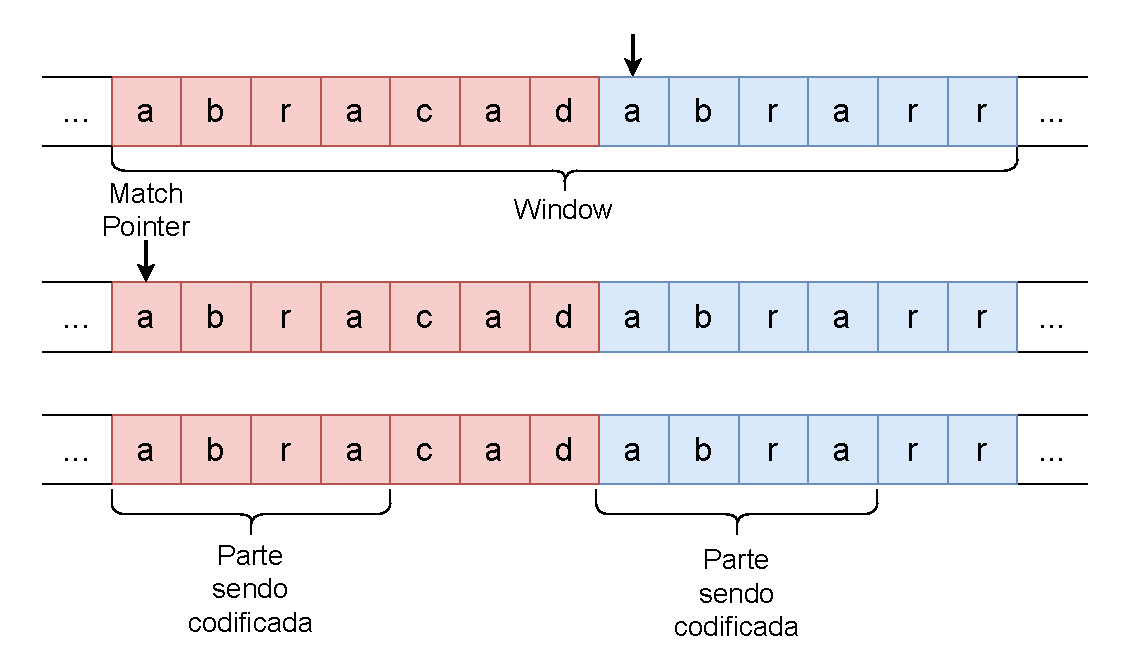
\includegraphics[width=15cm]{figuras/DiagramasTCC-LZ77-Estado-1.pdf}
  \fonte{Adaptada de \textcite{sayood2012introduction}}
\end{figure}

Nesse novo estado, procura-se novamente uma correspondência no \textit{search
  buffer} para a sequência do \textit{lookahead buffer}, que agora começa com
\texttt{"a"}. Observando o \textit{search buffer}, é possível encontrar
múltiplas ocorrências isoladas do caractere \texttt{"a"}, próximo a esquerda. Notavelmente, existe uma
sequência completa \texttt{"abra"} previamente codificada, iniciando a
0~caracteres de distância da posição atual da janela. Essa correspondência
possui comprimento 4~caracteres.

Dessa forma, o algoritmo codifica a sequência encontrada como o token $\langle
  0, 4, \texttt{r} \rangle$, onde $0$ indica a distância até o início da
correspondência no \textit{search buffer}, $4$ indica o comprimento da
correspondência encontrada (\texttt{"abra"}), e \texttt{"r"} é o caractere
seguinte imediatamente após essa sequência, ainda não codificado. Após isso, a
janela avança em 5~posições (4~caracteres da sequência codificada mais
1~caractere literal).

Para realizar o processo inverso, ou seja, decodificar o token recebido
$\langle 0, 4, \texttt{r} \rangle$, o decodificador utiliza o mesmo princípio
do algoritmo LZ77, porém no sentido inverso.

Inicialmente, ele utiliza o offset ($o$) para retornar exatamente 0 posições na
sequência já decodificada até o momento. A partir dessa posição inicial
encontrada, copia-se uma sequência de comprimento 4 (valor $l$), obtendo o
trecho \texttt{"abra"}. Em seguida, adiciona-se ao final desta sequência
copiada o caractere literal adicional ($c$), que neste exemplo é \texttt{"r"}.

Esse processo é ilustrado passo a passo na Figura~\ref{fig:Estado_deconding}.
Inicialmente, há o estado parcial da decodificação com o \textit{buffer} já
reconstruído. Em seguida, avança-se caractere a caractere, copiando-se do
\textit{buffer} reconstruído e adicionando o caractere literal no final. O
resultado final após a decodificação deste token será \texttt{"abrar"}.

Vale destacar que o decodificador reconstrói o buffer de busca dinamicamente,
conforme recebe e processa novos tokens, permitindo a reconstrução exata dos
dados originais sem perda alguma.

% Até Aqui

\begin{figure}[htp]
  \centering
  \caption{Decodificação do exemplo $\langle 7, 4, \texttt{r} \rangle$ }
  \label{fig:Estado_deconding}
  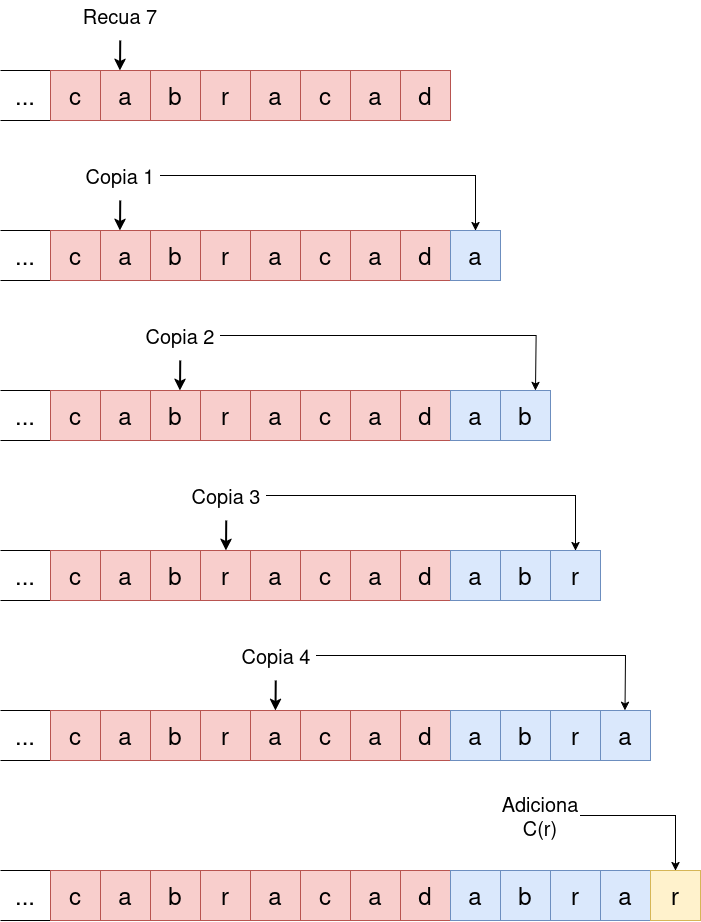
\includegraphics[width=12cm]{figuras/DiagramasTCC-LZ77-Decoding}
  \fonte{Adaptada de \textcite{sayood2012introduction}}
\end{figure}

Utilizando o exemplo anterior do token $\langle 7, 4, \texttt{r} \rangle$, onde
a janela total possui 13 caracteres, temos a seguinte definição dos campos em
bits:
\begin{itemize}
  \item O deslocamento ($p$) pode variar de 0 a 6, portanto requer $3$~bits;
  \item  O comprimento ($\ell$) pode variar de 0 a 7, logo exige também $3$~bits;
  \item O caractere literal ($c$) é codificado em ASCII, utilizando $8$~bits
        ($1$~byte).
\end{itemize}
Dado que na implementação adotada os tamanhos em bits para cada campo do token são
\[
  \underbrace{3}_{\substack{\text{bits para}\\\text{pointer }($p$)}} +
  \underbrace{3}_{\substack{\text{bits para}\\\text{length }(\ell)}} +
  \underbrace{8}_{\substack{\text{bits para}\\\text{character }(x)}}
  = 14\;\text{bits},
\]
temos um formato de código de comprimento fixo, no qual cada token $\langle p,
  \ell, x\rangle$ ocupará exatamente 14 bits. Em outras palavras, após definido o
tamanho da janela (\textit{pointer}) e do \textit{lookahead buffer}
(\textit{length}), bem como o padrão de 8 bits para o caractere literal, toda e
qualquer codificação produzida por esse esquema terá comprimento contínuo de 14
bits por símbolo codificado \cite{nelson2008data}.

Realizando a codificação especificamente para o exemplo dado ($\langle 0, 4,
  \texttt{r} \rangle$), obtêm-se:
\begin{itemize}
  \item O valor do \textit{offset} $o = 0$, em $3$ bits é $000_{(2)}$.
  \item O comprimento $l = 4$, em $3$ bits é $100_{(2)}$.
  \item O caractere $r$, em ASCII binário ($8$ bits), é $01110010_{(2)}$.
\end{itemize}
Portanto, a representação completa do token em bits será:
$$
  000 \;|\; 100 \;|\; 01110010
$$
Resultando na sequência binária final: $00010001110010_{(2)}$.

Esse processo ilustra o funcionamento fundamental do algoritmo LZ77, mostrando
como ele explora redundâncias por meio de correspondências encontradas em
trechos já codificados, reduzindo o volume de dados transmitidos ou
armazenados.

% Revisões Aqui
\newpage
\section{Biblioteca Komm}
A \textit{Komm} é uma biblioteca em \textit{Python} para sistemas de
comunicação desenvolvida pelo professor Roberto Nobrega. Trata-se de um projeto
\textit{open-source} para \textit{Python 3} que fornece ferramentas para
análise e simulação de sistemas de comunicação analógicos e digitais.

Este projeto foi inspirado em diversas outras bibliotecas para sistemas de
comunicação, como \textit{MATLAB\textsuperscript{\textregistered}
  Communications System Toolbox\texttrademark}, \textit{GNU Radio},
\textit{CommPy} e \textit{SageMath}.

Além disso, a biblioteca já disponibiliza diversas codificações implementadas,
abrangendo diferentes técnicas de \textit{source coding} e \textit{lossless
  coding}, incluindo:
\begin{itemize}
  \item {Shannon Code}
  \item {Fano Code}
  \item {Huffman Code}
  \item {Tunstal lCode}
  \item {LZ78}
  \item {LZW}
\end{itemize}
